\documentclass[11pt]{article}
\usepackage[a4paper, margin=1in]{geometry}
\usepackage{amsmath, amssymb}
\usepackage{hyperref}
\usepackage{graphicx}
\usepackage{titlesec}
\usepackage{listings} 
\usepackage{xcolor}   
\usepackage[utf8]{inputenc}
\usepackage{tikz}
\usepackage[T1]{fontenc}
\usepackage[numbers,sort&compress]{natbib}
\bibliographystyle{unsrtnat}
\usetikzlibrary{arrows.meta, positioning, shapes.geometric}

\title{Lecture notes}
\author{}
\date{}

\titleformat{\section}{\large\bfseries}{\thesection}{1em}{}
\titleformat{\subsection}{\normalsize\bfseries}{\thesubsection}{1em}{}

\begin{document}

\setlength{\parindent}{0pt}
\setlength{\parskip}{1ex}

\maketitle

\tableofcontents

\newpage
\section{Introducción}
\subsection{Motivación: Desafíos de la inferencia cosmológica moderna}
La cosmología observacional enfrenta una coyuntura crítica impulsada por la explosión en la cantidad y complejidad de los datos disponibles. Experimentos recientes como \textit{Planck} \citep{Planck2018} y Simons Observatory \citep{SO2019}, junto con proyectos futuros como CMB-S4 \citep{CMB-S42016}, generan conjuntos de datos cuyo análisis exhaustivo mediante métodos tradicionales basados en cadenas de Markov (MCMC) requiere recursos computacionales prohibitivos. Un caso emblemático es el análisis de los datos de \textit{Planck} 2018, que necesitó más de 10 millones de muestras MCMC para alcanzar convergencia en espacios de parámetros de más de 30 dimensiones \citep{Planck2018}, con un coste escalando como $\mathcal{O}(N^3)$ para $N$ modos observados \citep{Schneider2020}. Esta barrera computacional se agudizará en la próxima generación de experimentos con resoluciones angulares sub-arcminuto.

Paralelamente, la reducción de errores estadísticos por debajo del 1\% en mediciones de polarización \citep{BICEP2021} ha expuesto limitaciones fundamentales en el paradigma de inferencia actual. Errores sistemáticos anteriormente despreciables, tanto instrumentales (ruido correlacionado, efectos de haz asimétrico) como teóricos (no-Gaussianidad primordial, efectos de segundo orden en transferencia radiativa \citep{Challinor2011}), dominan ahora las incertidumbres. Particularmente problemática resulta la creciente evidencia de desviaciones de Gaussianidad en pequeños escalones angulares ($\ell > 2000$), donde los efectos de lente gravitacional distorsionan significativamente las estadísticas del fondo cósmico de microondas \citep{Planck2018NL}. Estas complejidades se amplifican al considerar análisis conjuntos de múltiples estadísticos como $C_\ell^{TT}$, $C_\ell^{TE}$ y funciones de correlación $\xi_+(\theta)$, cuyas covarianzas cruzadas introducen no-linearidades no triviales \citep{EFS2004}.

Este panorama exige desarrollar frameworks de inferencia alternativos que superen tres limitaciones clave: primero, la incapacidad de los métodos basados en likelihood exacto para escalar a los volúmenes de datos futuros; segundo, la dependencia crítica de aproximaciones Gaussianas cada vez más cuestionables; y tercero, la dificultad para incorporar sistemáticos complejos en modelos analíticos. La inferencia basada en simulaciones (SBI) emerge como solución prometedora al integrar emuladores de alta dimensión \citep{Alsing2019}, técnicas de compresión óptima de datos \citep{Jeffrey2021} y algoritmos de muestreo eficiente \citep{Papamakarios2019}, permitiendo una caracterización rigurosa de parámetros cosmológicos directamente desde observaciones sin necesidad de likelihoods explícitos.


\section{Statistics in cosmology}
Los cosmólogos enfrentan nuevos desafíos en el análisis de datos debido al crecimiento exponencial en la cantidad y calidad de información disponible. Experimentos recientes generan conjuntos de datos masivos que requieren métodos avanzados, ya que algoritmos tradicionales se vuelven ineficientes. Además, al reducirse los errores estadísticos, emergen errores sistemáticos previamente enmascarados, relacionados tanto con artefactos instrumentales como con limitaciones teóricas.

En esta introducción se presentan técnicas para el análisis cosmológico moderno, comenzando con conceptos estadísticos básicos (verosimilitud, previos y posteriores) y su aplicación a espectros de potencia. Introduce herramientas como la \textit{Matriz de Fisher} (para estimación rápida de errores) y métodos \textit{Markov Chain Monte Carlo} (MCMC), que permiten manejar verosimilitudes complejas. Estas metodologías, aunque desarrolladas para cosmología, tienen aplicaciones transversales en diversas áreas científicas que trabajan con grandes volúmenes de datos.

\subsection{The Likelihood function}
La función de verosimilitud $L(\{d_i\}|\theta)$ representa el núcleo conceptual de los análisis estadísticos modernos en cosmología. Se define formalmente como la probabilidad condicional de observar un conjunto de datos experimentales $\{d_i\}_{i=1}^m$ dado un modelo teórico parametrizado por $\theta = (w, \sigma_w)$. Para mediciones independientes, esta función se expresa como el producto de probabilidades individuales:

\begin{equation}
L(\{d_i\}|\theta) = \prod_{i=1}^m P(d_i|\theta), 
\end{equation}

donde cada término $P(d_i|\theta)$ corresponde a la distribución de probabilidad del modelo para cada dato observado. La potencia analítica de este constructo matemático reside en su capacidad para invertir la relación lógica entre datos y teoría mediante la aplicación del teorema de Bayes:

\begin{equation}
P(\theta|\{d_i\}) \propto L(\{d_i\}|\theta) P(\theta),
\end{equation}

permitiendo inferir los parámetros del modelo a partir de las observaciones. En el contexto del ejemplo pedagógico: -la medición del peso $w$ de un individuo utilizando $m=100$ básculas independientes con error gaussiano-, cada observación $d_i$ sigue una distribución normal $d_i \sim \mathcal{N}(w,\sigma_w^2)$. La verosimilitud para una sola medición adopta la forma gaussiana clásica:

\begin{equation}
L(d_i|w,\sigma_w) = (2\pi\sigma_w^2)^{-1/2} \exp\left(-\frac{(d_i - w)^2}{2\sigma_w^2}\right).
\end{equation}

Al extenderse a múltiples observaciones independientes, la verosimilitud conjunta se factoriza en un producto de términos gaussianos, lo que en escala logarítmica se traduce en una suma cuadrática: 

\begin{equation}
\ln L(\{d_i\}|w,\sigma_w) = -\frac{m}{2}\ln(2\pi\sigma_w^2) - \frac{1}{2\sigma_w^2}\sum_{i=1}^m (d_i - w)^2.
\end{equation}

Los estimadores de máxima verosimilitud (MLE) para los parámetros se obtienen mediante la optimización de esta función. Para el peso $w$, la condición $\partial \ln L/\partial w = 0$ conduce al estimador: 

\begin{equation}
\hat{w} = \frac{1}{m}\sum_{i=1}^m d_i,
\end{equation}

que corresponde a la media muestral. Análogamente, al resolver $\partial \ln L/\partial \sigma_w^2 = 0$ se obtiene el estimador para la varianza 

\begin{equation}
\hat{\sigma}_w^2 = \frac{1}{m}\sum_{i=1}^m (d_i - \hat{w})^2.
\end{equation} 

Estos resultados ejemplifican cómo los principios de máxima verosimilitud recuperan estimadores intuitivos en casos simples. La transición desde la verosimilitud hacia la distribución posterior de parámetros se realiza mediante el teorema de Bayes:

\begin{equation}
P(w,\sigma_w|\{d_i\}) \propto L(\{d_i\}|w,\sigma_w) P_{\text{prior}}(w,\sigma_w),
\end{equation}

donde $P_{\text{prior}}$ incorpora cualquier conocimiento a priori sobre los parámetros. Esta distribución posterior contiene toda la información probabilística sobre los parámetros condicionada a los datos observados. La constante de normalización, denominada evidencia, asegura que la posterior integre a unidad sobre el espacio de parámetros. El análisis de incertidumbres en los estimadores se fundamenta en el examen de la curvatura del logaritmo de la verosimilitud alrededor de su máximo. Para el parámetro $w$, la varianza del estimador resulta:

\begin{equation}
\text{Var}(\hat{w}) =\frac{\sigma_w^2}{m},
\end{equation}

reflejando la reducción clásica de ruido conforme $\sqrt{m}$. En contraste, la estimación de $\sigma_w^2$ presenta comportamientos no-gaussianos, con varianza:

\begin{equation}
\text{Var}(\hat{\sigma}_w^2) = \frac{2}{m}\sigma_w^4.
\end{equation}

Este error en $\sigma_w$ puede parecer un detalle técnico, pero en cosmología, gran parte de lo que medimos (como fluctuaciones en la densidad de galaxias o la temperatura del CMB) es análogo a $\sigma_w^2$. Estas fluctuaciones siguen distribuciones (a menudo gaussianas) cuyos parámetros dependen del modelo cosmológico. Por ello, esta ecuación es fundamental: al estimar la varianza de una distribución, hay una incertidumbre intrínseca proporcional a $\sigma_w^2 / \sqrt{m}$, llamada varianza muestral o varianza cósmica. 

Por otro lado, es conveniente definir intervalos de credibilidad para los parámetros. En el ejemplo de la verosimilitud gaussiana, los intervalos de confianza al $68\%$ (1-$\sigma$) corresponden a la región donde $\ln L$ decrece en $1/2$ unidades desde su valor máximo, delimitando así el rango de parámetros consistentes con los datos. De manera general, se definen los valores $\omega_-$ y $\omega_+$ tales que:

\begin{equation}
\int_{\omega_-}^{\omega_+}d\omega P(\omega|\{d_i\}) = 0.68,
\end{equation}

En aplicaciones reales, usualmente hay múltiples parámetros desconocidos. Si algunos son irrelevantes, debemos marginalizar sobre ellos, formalmente esto se implementa mediante la integración multidimensional: 

\begin{equation}
P(\theta|\{d_i\}) = \int_{\Phi} P(\theta,\phi|\{d_i\}) d\phi,
\end{equation}

sobre el espacio completo $\Phi$ de parámetros \textit{nuisance}.

\subsection{From raw data to parameter constraints}

\begin{figure}[htbp]
    \centering
    \resizebox{0.95\textwidth}{!}{
    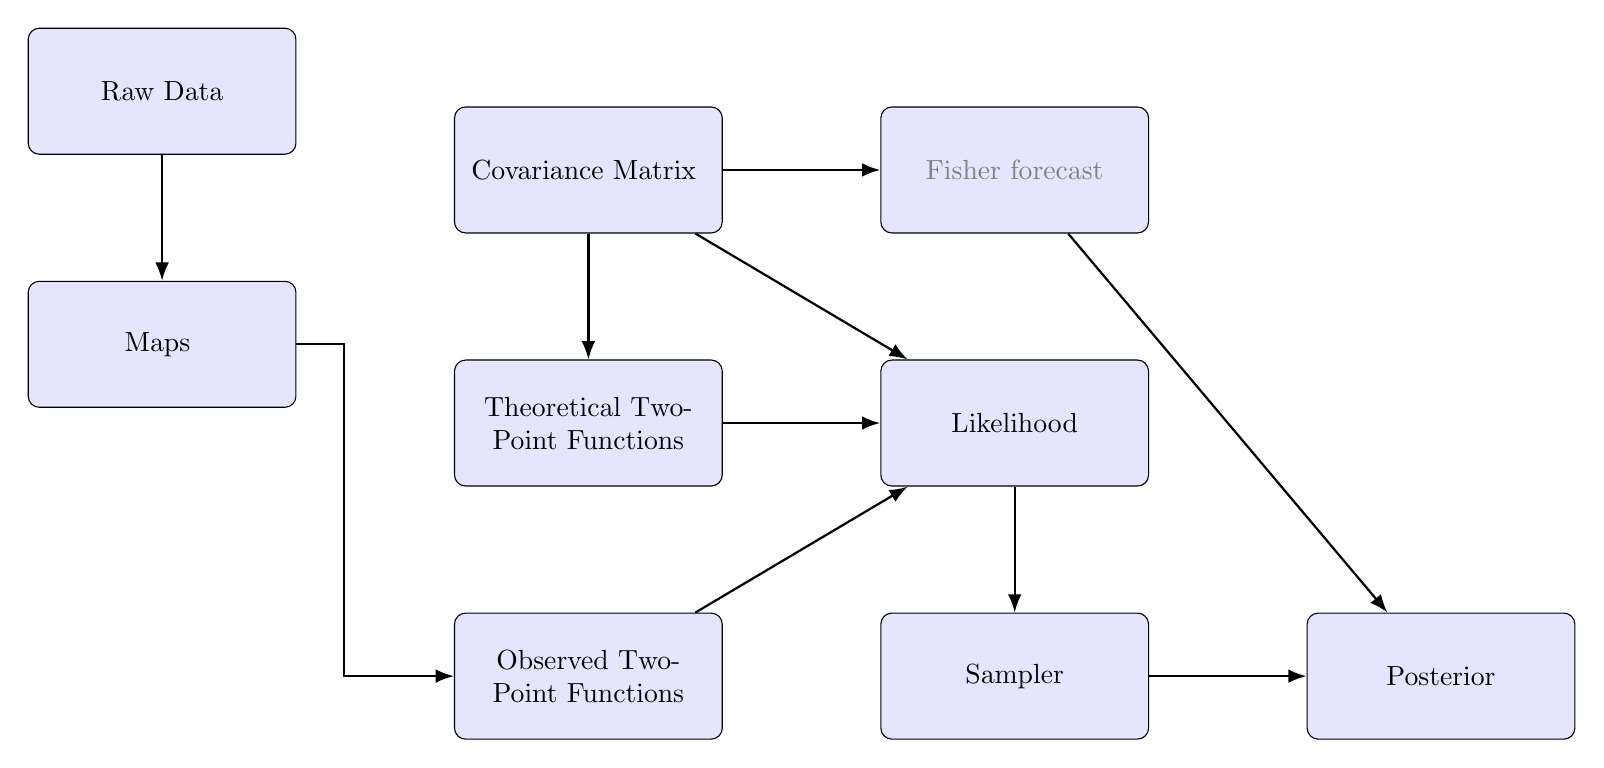
\begin{tikzpicture}[
        node distance=1.6cm and 2cm,
        box/.style={
            draw, 
            rounded corners, 
            minimum width=3.4cm, 
            minimum height=1.6cm, 
            align=center, 
            fill=blue!10
        },
        arrow/.style={-{Latex}, thick}
    ]
        % Nodes
        \node[box] (raw) {Raw Data};
        \node[box, below=of raw] (maps) {Maps };
        \node[box, right=of raw, yshift=-1cm] (cov) {Covariance Matrix };
        \node[box, below=of cov] (theory) {Theoretical Two-\\Point Functions};
        \node[box, below=of theory] (obs) {Observed Two-\\Point Functions};
        \node[box, right=of theory] (like) {Likelihood};
        \node[box, below=of like] (sampler) {Sampler};
        \node[box, right=of sampler] (posterior) {Posterior};

        % Optional forecast box (light gray text)
        \node[box, above=of like, text=gray] (fisher) {Fisher forecast};

        % Arrows
        \draw[arrow] (raw) -- (maps);
        \draw[arrow] (maps.east) -- ++(0.6,0) |- (obs.west);
        \draw[arrow] (cov) -- (like);
        \draw[arrow] (obs) -- (like);
        \draw[arrow] (theory) -- (like);
        \draw[arrow] (like) -- (sampler);
        \draw[arrow] (sampler) -- (posterior);
        \draw[arrow, thick] (cov) -- (fisher);
        \draw[arrow, thick] (fisher) -- (posterior);
        \draw[arrow] (cov) -- (theory);
    \end{tikzpicture}
    }
    \caption{Pipeline desde los datos crudos hasta las restricciones cosmológicas.}
    \label{fig:pipeline_cosmo}
\end{figure}

El análisis cosmológico moderno sigue una metodología bien establecida que comienza con los mapas observacionales. Estos representan la materia prima del estudio, correspondiendo a representaciones espaciales de los fenómenos cósmicos investigados. En el caso de la radiación cósmica de fondo (CMB), se trabaja con mapas de anisotropías de temperatura; para sondeos galácticos, con distribuciones tridimensionales de densidad; y en estudios de lente gravitacional débil, con campos de elipticidad galáctica.

A partir de estos mapas, se extraen los estadísticos de dos puntos, que capturan las correlaciones fundamentales mediante funciones de dos puntos. Estas pueden expresarse tanto en el espacio espectral como en el espacio de configuraciones, proporcionando así una descripción estadística compacta de las propiedades de los campos observados. La transición de los mapas brutos a estos estadísticos permite reducir considerablemente la dimensionalidad de los datos, reduciendo la complejidad computacional, pero perdiendo información no gaussiana.

Con los estadísticos medidos en mano, el siguiente paso es la construcción de la verosimilitud, que compara estas mediciones con sus contrapartes teóricas. Esta comparación se realiza ponderando las diferencias mediante la matriz de covarianza inversa. Para el caso gaussiano, la función de verosimilitud para las anisotropías del CMB toma la forma:

\begin{equation}
\ln \mathcal{L}(\lambda_\alpha) = -\frac{1}{2} \sum_{ll'} \left( \hat{C}(l) - C_{\text{theory}}(l, \lambda_\alpha) \right) \text{Cov}^{-1}_{ll'} \left( \hat{C}(l') - C_{\text{theory}}(l', \lambda_\alpha) \right)
\end{equation}

Para explorar el espacio de parámetros cosmológicos $\lambda_\alpha$ se emplean técnicas de muestreo de parámetros, particularmente algoritmos MCMC (Monte Carlo Markov Chain). Estos algoritmos evalúan sistemáticamente millones de combinaciones paramétricas, permitiendo caracterizar completamente la distribución posterior. Este proceso debe manejar adecuadamente dos desafíos clave: las degeneraciones entre parámetros cosmológicos y la marginalización sobre parámetros molestos no cosmológicos, como el parámetro de bias $b_1$ en estudios de distribución galáctica.

Como complemento al muestreo exhaustivo, las estimaciones analíticas mediante pronósticos de Fisher ofrecen una alternativa eficiente para proyectar barras de error. Estas aproximaciones analíticas son especialmente valiosas en etapas preliminares de diseño experimental, cuando se requiere evaluar rápidamente el potencial científico de diferentes configuraciones instrumentales sin recurrir a costosos análisis completos. El proceso completo se ilustra en la Figura~\ref{fig:pipeline_cosmo}.





\clearpage

\section{Introducciónnn}
\subsection{Motivación}
La inferencia sin verosimilitud (\textit{likelihood-free inference}) permite estimar parámetros cosmológicos sin asumir una forma analítica para la función de verosimilitud, evitando así sesgos por supuestos incorrectos como Gaussianidad. Esto es especialmente relevante en cosmología, donde procesos no lineales y efectos sistemáticos complican el modelado estadístico. En el contexto del CMB, aunque las fluctuaciones primordiales son aproximadamente Gaussianas, efectos secundarios, como lentes gravitacionales, polarización inducida y \textit{foregrounds} introducen no-Gaussianidades que desafían los análisis tradicionales basados en espectros de potencia.

El CMB es uno de los observables más poderosos para estudiar los parámetros cosmológicos, pero su buena explotación requiere ir más allá de las estadísticas de dos puntos. En este trabajo, comenzaré con el análisis de estadísticas resumidas tradicionales, partiendo de los \textit{angular power spectrum} (APS) de temperatura, que capturan la información gaussiana primordial. Posteriormente, escalaré hacia estadísticas más complejas que incluyan modos de polarización, para finalmente explorar métodos no lineales (de ser posible).

Métodos de aprendizaje profundo, como la compresión neuronal, pueden extraer información no lineal de mapas del CMB, mejorando las restricciones sobre parámetros como $\Omega_m$ o $\sigma_8$. Además, la inclusión de efectos no ideales como ruido instrumental, cortes en el cielo y \textit{foregrounds} en simulaciones realistas es importante para un análisis robusto. Esta aproximación gradual---desde espectros de potencia hasta estadísticas de alto orden---permitirá validar resultados intermedios y cuantificar ganancias al incorporar información no gaussiana.

\subsection{Inferencia Bayesiana}
El marco bayesiano permite determinar la distribución posterior de parámetros cosmológicos $\theta$ mediante la expresión 

\begin{equation}
p(\theta|x) = \frac{p(x|\theta)p(\theta)}{p(x)}
\end{equation}

donde $x$ representa los datos observacionales. La determinación precisa de la función de verosimilitud $p(x|\theta)$ presenta varios desafíos en el análisis del CMB. Aunque las fluctuaciones primordiales son aproximadamente gaussianas, efectos secundarios como las lentes gravitacionales, la contaminación por \textit{foregrounds} y las no-linearidades instrumentales introducen complejidades. Estas complicaciones se acentúan al considerar estadísticas más allá del espectro de potencia, como los estudios de no-gaussianidad primordial o los análisis de lentes gravitacionales a pequeña escala.

Los métodos tradicionales basados en supuestos gaussianos para la verosimilitud muestran limitaciones crecientes frente a la precisión de los nuevos experimentos. Particularmente, para análisis que involucran reconstrucción de lentes, estudios de no-gaussianidad o el tratamiento de regiones con máscaras complejas, la distribución exacta de los estadísticos se desvía significativamente de la aproximación gaussiana. Esta discrepancia puede llevar a estimaciones sesgadas de parámetros cosmológicos.

\subsection{\textit{Likelihood-free inference}}
La inferencia sin verosimilitud (también llamada \textit{Simulation-based inference}) busca realizar inferencia estadística en situaciones donde la función de verosimilitud es intratable o desconocida. Métodos tradicionales como el \textit{Approximate Bayesian Computation} (ABC) abordan este problema comparando directamente los datos simulados con los datos observados mediante una métrica de distancia. En este enfoque, se generan múltiples simulaciones a partir de diferentes valores del parámetro $\theta$ y se conservan aquellos para los cuales los datos simulados $x$ se parecen lo suficiente a los datos observados, según un umbral de tolerancia. Este método depende fuertemente de la elección de estadísticas resumidas y puede requerir un número muy elevado de simulaciones para obtener una aproximación razonable de la distribución posterior. La figura 1 se muestra la pipeline general utilizada para estimar posteriores con el método ABC.

\begin{figure}[htbp]
    \centering
    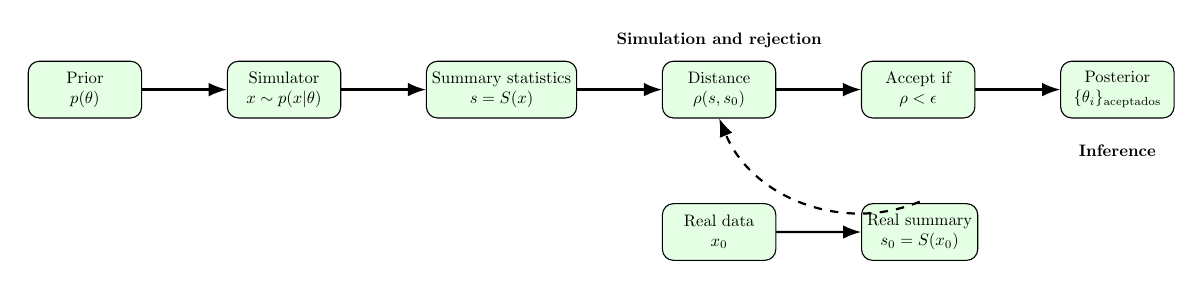
\begin{tikzpicture}[
        scale=0.6,
        every node/.style={transform shape},
        node distance=1.2cm and 1.8cm,
        box/.style={draw, rounded corners, minimum width=2.4cm, minimum height=1.2cm, align=center, fill=green!10},
        arrow/.style={-{Latex}, thick}
    ]
        \node[box] (prior) {Prior \\ \( p(\theta) \)};
        \node[box, right=of prior] (simulator) {Simulator \\ \( x \sim p(x|\theta) \)};
        \node[box, right=of simulator] (summary) {Summary statistics \\ \( s = S(x) \)};
        \node[box, right=of summary] (distance) {Distance \\ \( \rho(s, s_0) \)};
        \node[box, right=of distance] (accept) {Accept if \\ \( \rho < \epsilon \)};
        \node[box, below=1.8cm of distance] (obs) {Real data \\ \( x_0 \)};
        \node[box, right=of obs] (s_obs) {Real summary \\ \( s_0 = S(x_0) \)};
        \node[box, right=of accept] (posterior) {Posterior \\ \( \{\theta_i\}_{\text{aceptados}} \)};

        \draw[arrow] (prior) -- (simulator);
        \draw[arrow] (simulator) -- (summary);
        \draw[arrow] (summary) -- (distance);
        \draw[arrow] (distance) -- (accept);
        \draw[arrow] (accept) -- (posterior);
        \draw[arrow] (obs) -- (s_obs);
        \draw[arrow, dashed] ([yshift=1pt] s_obs.north) to[bend left=45] (distance.south);

        \node[above=0.15cm of distance] {\textbf{Simulation and rejection}};
        \node[below=0.45cm of posterior] {\textbf{Inference}};
    \end{tikzpicture}
    \caption{Pipeline general de ABC.}
    \label{fig:abc}
\end{figure}

Más recientemente, técnicas modernas basadas en aprendizaje automático han revolucionado este enfoque. En lugar de comparar datos de manera directa, estos métodos reformulan el problema como uno de estimación de densidad: se modela la distribución conjunta de pares $(\theta, x)$ simulados, lo que permite aproximar la distribución posterior $p(\theta|x)$. Herramientas como redes neuronales profundas y flujos normalizantes permiten entrenar modelos expresivos que aprenden directamente la relación entre datos y parámetros a partir de muestras sintéticas, evitando el cálculo explícito de la verosimilitud y haciendo la inferencia mucho más eficiente. La figura 2 muestra la pipeline general para técnicas de sbi basadas en aprendizaje automático.

\begin{figure}[htbp]
    \centering
    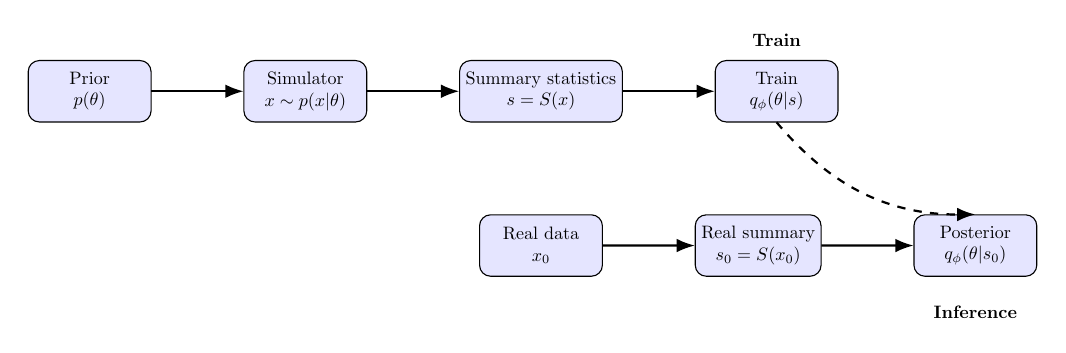
\begin{tikzpicture}[
        scale=0.65,  
        every node/.style={transform shape}, 
        node distance=1.2cm and 1.8cm,
        box/.style={draw, rounded corners, minimum width=2.4cm, minimum height=1.2cm, align=center, fill=blue!10},
        arrow/.style={-{Latex}, thick}
    ]
        \node[box] (prior) {Prior \\ \( p(\theta) \)};
        \node[box, right=of prior] (simulator) {Simulator \\ \( x \sim p(x|\theta) \)};
        \node[box, right=of simulator] (summary) {Summary statistics \\ \( s = S(x) \)};
        \node[box, right=of summary] (train) {Train \\ \( q_\phi(\theta|s) \)};
        \node[box, below=1.8cm of summary] (obs) {Real data \\ \( x_0 \)};
        \node[box, right=of obs] (s_obs) {Real summary \\ \( s_0 = S(x_0) \)};
        \node[box, right=of s_obs] (posterior) {Posterior \\ \( q_\phi(\theta|s_0) \)};

        \draw[arrow] (prior) -- (simulator);
        \draw[arrow] (simulator) -- (summary);
        \draw[arrow] (summary) -- (train);
        \draw[arrow] (obs) -- (s_obs);
        \draw[arrow] (s_obs) -- (posterior);
        \draw[arrow, dashed] (train.south) to[bend right=25] (posterior.north);

        \node[above=0.15cm of train] {\textbf{Train}};
        \node[below=0.45cm of posterior] {\textbf{Inference}};
    \end{tikzpicture}
    \caption{Pipeline general para métodos con aprendizaje automático.}
    \label{fig:sbi}
\end{figure}

El paquete \texttt{sbi}, desarrollado en Python sobre \texttt{PyTorch}, implementa este paradigma de manera flexible. Ofrece herramientas para: (1) simular datos bajo distintos parámetros $\theta$, (2) entrenar estimadores de densidad condicional $p(\theta|x)$ usando arquitecturas modernas, y (3) realizar inferencia posterior dado un conjunto de datos observados. La calidad de las simulaciones y de las estadísticas utilizadas continúa siendo muy importante, ya que el modelo entrenado sólo puede aprender lo que está presente en los datos simulados. Sin embargo, al entrenar modelos que generalizan bien, se puede reducir de forma significativa el número de simulaciones necesarias, logrando una inferencia más precisa y escalable que con métodos como ABC.

\section{Simulador}
\subsection{Generador de APS}
El generador implementa un cálculo teórico completo de las anisotropías del fondo cósmico de microondas mediante la resolución numérica de las ecuaciones de Boltzmann a través del código \texttt{CAMB}. Parte de un conjunto de parámetros cosmológicos que definen un modelo $\Lambda$CDM estándar y devuelve su \textit APS correspondiente. En la actual implementación, el cálculo se restringe al espectro de temperatura, aunque la arquitectura del código permite una extensión futura para incluir los modos de polarización. El resultado final consiste en el APS completo expresado en microkelvin, que cuantifica las fluctuaciones de temperatura en función del multipolo $\ell$. 

\subsection{Ruido instrumental y cobertura parcial del cielo}
Para generar simulaciones realistas de los APS, se consideran dos fuentes principales de ruido: el ruido instrumental del experimento y la cobertura parcial del cielo, que introduce varianza cósmica adicional. Primero, se añade el ruido instrumental a los espectros teóricos mediante un modelo basado en la resolución angular del experimento (\(\theta_{\text{fwhm}}\)) y la sensibilidad por píxel (\(\sigma_T\)). El término de ruido instrumental \(N_\ell^{\mathrm{TT}}\) que se suma al espectro de potencia teórico \(C_\ell\) es:

\begin{equation}
N_\ell^{\mathrm{TT}} = \left(\theta_{\text{fwhm}} \cdot \sigma_T \right)^2 \exp\left[ \ell (\ell + 1) \frac{\theta_{\text{fwhm}}^2}{8 \ln 2} \right],
\end{equation}

donde \(\theta_{\text{fwhm}}\) se expresa en radianes. Esta fórmula modela el suavizado del cielo debido a la resolución finita del instrumento. Posteriormente, se simula la observación del cielo parcial considerando que solo se mide una fracción \(f_{\text{sky}} < 1\) del cielo completo. Como consecuencia, el estimador observable de \(C_\ell\), denotado \(\hat{C}_\ell\), no es determinístico, sino una variable aleatoria cuya dispersión depende de \(f_{\text{sky}}\). Para multipolos bajos (\(\ell < \ell_{\text{transition}}\)), se modela esta varianza como una distribución chi-cuadrado escalada:

\begin{equation}
\hat{C}_\ell = \frac{1}{\nu_\ell} \sum_{i=1}^{\nu_\ell} X_i^2, \quad X_i \sim \mathcal{N}(0, \sqrt{C_\ell}),
\end{equation}

donde \(\nu_\ell = \text{round}(f_{\text{sky}} \cdot (2\ell + 1))\) representa el número efectivo de grados de libertad. Esta formulación captura correctamente la dispersión estadística del estimador cuando el número de modos disponibles es pequeño. Para multipolos altos (\(\ell \geq \ell_{\text{transition}}\)), se asume que el estimador puede aproximarse mediante una distribución normal centrada en \(C_\ell\) con varianza:

\begin{equation}
\hat{C}_\ell \sim \mathcal{N}\left(C_\ell, \frac{2 C_\ell^2}{f_{\text{sky}} (2\ell + 1)} \right).
\end{equation}

Este enfoque es válido debido al teorema central del límite, ya que en esta región el número de modos es suficientemente grande como para justificar una aproximación gaussiana.

\section{Inference}

\newpage
\section{Métodos bayesianos}
En las últimas décadas, la cosmología ha experimentado una explosión en la cantidad y calidad de datos observacionales, desde mediciones de anisotropías en el Fondo Cósmico de Microondas (CMB) hasta sondeos de galaxias y lentes gravitacionales a gran escala. Este crecimiento ha impulsado la necesidad de técnicas de análisis más sofisticadas, capaces de manejar conjuntos de datos masivos y modelos teóricos cada vez más complejos.  

En este contexto, los métodos bayesianos se han convertido en una herramienta fundamental para la inferencia cosmológica. Estos permiten combinar observaciones con predicciones teóricas mediante el uso de distribuciones de probabilidad, actualizando nuestro conocimiento a través del teorema de Bayes:  

\begin{equation}  
    P(\theta \mid \mathcal{D}) = \frac{P(\mathcal{D} \mid \theta) \, P(\theta)}{P(\mathcal{D})},  
\end{equation}  

donde \( P(\theta \mid \mathcal{D}) \) es la distribución posterior, \( P(\mathcal{D} \mid \theta) \) es la verosimilitud, \( P(\theta) \) es la distribución previa, y \( P(\mathcal{D}) \) actúa como evidencia.  

Sin embargo, en cosmología, el cálculo de la verosimilitud suele ser computacionalmente costoso o incluso intratable cuando se trabaja con simulaciones numéricas. Esto ha llevado al desarrollo de técnicas de \textit{Simulation-Based Inference} (SBI), que evitan la evaluación explícita de la verosimilitud mediante aproximaciones basadas en simulaciones. En las siguientes secciones, exploraremos cómo estos métodos están revolucionando el análisis de datos cosmológicos.

\subsection{Función de verosimilitud}
La función de verosimilitud \( L \) es fundamental en análisis estadísticos modernos, definida como la probabilidad de observar los datos dado un modelo teórico. Esta herramienta permite estimar parámetros del modelo y sus incertidumbres. Por ejemplo, al medir repetidamente el peso de una persona con múltiples básculas, la verosimilitud modela cómo las mediciones \( d_i \) se distribuyen alrededor del peso real \( w \), asumiendo un ruido gaussiano con desviación estándar \( \sigma_w \).

\begin{equation}
L(w | d_i, \sigma_w) = \frac{1}{\sqrt{2 \pi \sigma_w^2}} \exp \left( -\frac{(d_i - w)^2}{2 \sigma_w^2} \right)
\end{equation}

Para \( m \) mediciones independientes, la verosimilitud conjunta es el producto de las verosimilitudes individuales, resultando en una expresión exponencial que depende de la suma de cuadrados de las diferencias entre datos y modelo.

\begin{equation}
L(w | d_i, \sigma_w) = \prod_i \frac{1}{\sqrt{2 \pi \sigma_w^2}} \exp \left( -\frac{(d_i - w)^2}{2 \sigma_w^2} \right)
\end{equation}

\bibliography{references}
\end{document}